% ============================================================
% Bao cao do an: Laplace's Demon — AI Agent ca nhan qua Telegram
%
% Bien dich:
%   latexmk -pdf main.tex
% hoac:
%   pdflatex main.tex && bibtex main && pdflatex main.tex && pdflatex main.tex
%
% Yeu cau goi tieng Viet: vntex + babel-vietnamese (co san trong TeX Live
% scheme-full; ban cai gon thi `tlmgr install vntex babel-vietnamese`).
% Khong co TeX local? Da kiem chung bien dich sach bang Docker:
%   docker run --rm -v "$PWD":/work -w /work texlive/texlive:latest \
%     latexmk -pdf -interaction=nonstopmode main.tex
%
% Cau truc: van de -> kien thuc nen -> kien truc -> ky thuat -> phuong phap
% thuc nghiem -> ket qua -> gioi han. Phan ket qua (sections/06_ket_qua.tex)
% la KHUNG cho so lieu — moi cho can dien danh dau bang \todo{...}, nguon so
% lieu: evals/results/exp-final (bang summary trong report.md / results.json).
% ============================================================
\documentclass[a4paper,12pt]{article}

\usepackage[utf8]{inputenc}
\usepackage[T5]{fontenc}
\usepackage[vietnamese]{babel}
\usepackage[margin=2.5cm]{geometry}
\usepackage{graphicx}
\usepackage{booktabs}      % bang dep (\toprule/\midrule/\bottomrule)
\usepackage{amsmath}
\usepackage{amssymb}   % \rightleftarrows trong so do trang thai
\usepackage{xcolor}
\usepackage{url}
\usepackage[hidelinks]{hyperref}
\usepackage{enumitem}
\setlist{nosep}

% Danh dau cho can dien so lieu thi nghiem (evals/results/exp-final).
% Khi hoan tat bao cao: thay het \todo{...} bang so lieu that; co the kiem tra
% con sot khong bang: grep -n "\\\\todo" sections/*.tex
\newcommand{\todo}[1]{\textcolor{red}{\textbf{[TODO: #1]}}}

% Duong dan hinh: xuat bieu do tu eval harness vao thu muc figures/
\graphicspath{{figures/}}

\title{\textbf{Laplace's Demon}\\
  \large AI Agent cá nhân qua Telegram:\\
  vòng lặp tự hành có quan sát được và đánh giá định lượng}
\author{Nguyễn Thành\thanks{Thông tin lớp/khoa/trường — điền sau.}}
\date{\today}

\begin{document}

\maketitle

\begin{abstract}
Báo cáo trình bày Laplace's Demon, một AI agent cá nhân nhận yêu cầu ngôn ngữ
tự nhiên qua Telegram và tự thực hiện vòng lặp phân tích --- lập kế hoạch ---
gọi công cụ --- quan sát --- điều chỉnh --- trả lời. Khác với các lớp vỏ gọi
API LLM, hệ thống đặt trọng tâm vào độ tin cậy (giới hạn bước, timeout, xác
nhận người dùng, trần chi phí mỗi tác vụ), khả năng quan sát (full execution
trace, trace viewer có chế độ phát lại) và đánh giá định lượng (eval harness
66 test case thuộc 8 nhóm, 8 metric, tùy chọn LLM-as-judge). Thực nghiệm so
sánh hai chiến lược điều phối (ReAct, Plan-and-Execute) trên hai cấu hình mô
hình ngôn ngữ (mock tất định và Gemini) theo ma trận $2 \times 2$ cho thấy
\todo{dien 1--2 cau ket qua chinh tu evals/results/exp-final}.
\end{abstract}

\tableofcontents
\clearpage

\section{Vấn đề}
\label{sec:van-de}

\subsection{Bối cảnh}

Các mô hình ngôn ngữ lớn (LLM) đã vượt qua vai trò công cụ hỏi--đáp: khi được
ghép với khả năng gọi công cụ (tool calling), chúng có thể \emph{hành động} ---
tìm kiếm thông tin, đọc trang web, ghi dữ liệu, lên lịch --- thay vì chỉ sinh
văn bản. Lớp hệ thống này thường được gọi là \emph{AI agent}: LLM đóng vai trò
bộ điều khiển, quyết định bước tiếp theo dựa trên yêu cầu của người dùng và
quan sát thu được từ môi trường~\cite{yao2023react}.

Tuy nhiên, khoảng cách giữa một bản demo agent và một hệ thống dùng được hằng
ngày là rất lớn. Ba vấn đề nổi bật:

\begin{enumerate}
  \item \textbf{Độ tin cậy.} LLM không tất định và có thể ``ảo giác'': chọn sai
        công cụ, bịa tên công cụ không tồn tại, lặp vô hạn, hoặc thực hiện hành
        động có hại (xóa dữ liệu) mà người dùng không hay biết. Một agent hữu
        dụng phải có các lớp chặn tường minh: giới hạn số bước, timeout, xác
        nhận của con người trước hành động ghi/xóa.
  \item \textbf{Khả năng quan sát.} Khi agent trả lời sai hoặc hành xử lạ, câu
        hỏi ``nó vừa làm gì và vì sao'' phải trả lời được. Đa số demo agent chỉ
        ghi log rời rạc; việc dựng lại toàn bộ chuỗi quyết định (prompt nào,
        công cụ nào, tham số gì, quan sát gì, tốn bao nhiêu token) thường là
        không thể.
  \item \textbf{Đánh giá định lượng.} Hành vi agent phụ thuộc mô hình, prompt
        và chiến lược điều phối. Không có bộ đo lặp lại được thì mọi thay đổi
        (đổi model, sửa prompt) đều là cảm tính --- không biết hệ thống tốt lên
        hay xấu đi.
\end{enumerate}

\subsection{Bài toán}

Đồ án đặt bài toán: xây dựng một \textbf{AI agent cá nhân} giao tiếp qua
Telegram, tự thực hiện trọn vẹn vòng lặp \emph{nhận yêu cầu $\to$ phân tích
$\to$ lập kế hoạch $\to$ gọi công cụ $\to$ quan sát $\to$ điều chỉnh $\to$ trả
lời} trên một bộ công cụ thực dụng (tìm kiếm web, đọc trang, ghi chú, việc cần
làm, viết báo cáo, lên lịch định kỳ), với ba yêu cầu xuyên suốt tương ứng ba
vấn đề trên:

\begin{itemize}
  \item \textbf{An toàn theo lớp}: giới hạn bước và timeout ở mọi tầng; hành
        động ghi/xóa phải qua xác nhận người dùng (human-in-the-loop) với cơ
        chế tạm dừng/tiếp tục bền vững qua restart.
  \item \textbf{Trace là công dân hạng nhất}: mọi lệnh gọi LLM và mọi lần chạy
        công cụ đều được ghi vào cơ sở dữ liệu; một trace viewer dựng lại được
        toàn bộ timeline kèm token, chi phí, độ trễ.
  \item \textbf{Đánh giá tự động}: một eval harness chạy bộ test case cố định
        qua chính agent loop production, chấm tự động và xuất bảng metric ---
        làm nền cho thí nghiệm so sánh chiến lược và mô hình.
\end{itemize}

Tên dự án lấy ẩn dụ từ thí nghiệm tư duy của Pierre-Simon Laplace về một thực
thể biết toàn bộ trạng thái hiện tại của vũ trụ và từ đó suy ra tương lai ---
ở đây tượng trưng cho nguyên tắc thiết kế: agent \emph{quyết định dựa trên
trạng thái quan sát được và được ghi lại đầy đủ}, chứ không phải tuyên bố hệ
thống ``biết mọi thứ''.

\subsection{Phạm vi và đóng góp}

Phạm vi MVP: một người dùng cá nhân (hoặc nhóm nhỏ), một tiến trình, kênh
Telegram, 6 công cụ, SQLite. Ngoài phạm vi: multi-agent, RAG/vector memory,
hạ tầng phân tán.

Đóng góp chính của đồ án:

\begin{enumerate}
  \item Một agent loop \textbf{tự xây dựng} (không dùng framework agent) dưới
        dạng state machine tường minh, hỗ trợ hai chiến lược điều phối cắm
        chung một interface: ReAct~\cite{yao2023react} và
        Plan-and-Execute~\cite{wang2023planandsolve};
  \item Cơ chế human-in-the-loop \textbf{bền vững}: trạng thái tạm dừng lưu
        trong DB, tiếp tục được ở tiến trình khác, chống thực thi kép bằng
        compare-and-set;
  \item Hệ thống trace đầy đủ + trace viewer, dùng chung một nguồn dữ liệu cho
        cả gỡ lỗi lẫn đánh giá;
  \item Eval harness với 37 test case thuộc 8 nhóm (bao gồm cả prompt
        injection và phục hồi lỗi), 9 metric, tùy chọn
        LLM-as-judge~\cite{zheng2023judge}; và thí nghiệm so sánh
        $2 \times 2$ (chiến lược $\times$ mô hình).
\end{enumerate}

\section{Kiến thức nền}
\label{sec:kien-thuc-nen}

Mục này trình bày các khái niệm và kỹ thuật nền tảng mà hệ thống dựa vào. Mỗi
khái niệm được nêu ngắn gọn kèm nguồn gốc; cách chúng được hiện thực hóa cụ
thể trong hệ thống trình bày ở Mục~\ref{sec:kien-truc}
và~\ref{sec:ky-thuat}.

\subsection{AI agent dựa trên LLM}

Một \emph{agent} dựa trên LLM là hệ thống trong đó mô hình ngôn ngữ đóng vai
trò bộ điều khiển trung tâm: nhận mục tiêu từ người dùng, quyết định hành động
kế tiếp (gọi công cụ nào, với tham số gì), quan sát kết quả và lặp lại cho đến
khi hoàn thành~\cite{wang2024agentsurvey}. Khác với chatbot hỏi--đáp một lượt,
agent duy trì \emph{trạng thái tác vụ} qua nhiều bước và tương tác với môi
trường bên ngoài. Nền tảng cho khả năng suy luận nhiều bước là kỹ thuật
chain-of-thought: yêu cầu mô hình sinh chuỗi lập luận trung gian trước khi
kết luận, giúp cải thiện đáng kể các bài toán cần nhiều bước
suy diễn~\cite{wei2022cot}.

\subsection{ReAct: đan xen suy luận và hành động}

ReAct (Reason + Act)~\cite{yao2023react} là khuôn mẫu điều phối trong đó mô
hình sinh xen kẽ ba loại phần tử: \emph{thought} (suy nghĩ về tình huống hiện
tại), \emph{action} (hành động --- thường là một lệnh gọi công cụ) và
\emph{observation} (quan sát trả về từ môi trường). Ở mỗi vòng, toàn bộ lịch
sử thought--action--observation được đưa lại vào ngữ cảnh để mô hình quyết
định bước kế tiếp: gọi thêm một công cụ hoặc đưa ra câu trả lời cuối. Ưu điểm
của ReAct là tính thích ứng --- mô hình ``nghĩ lại'' sau mỗi quan sát nên xử
lý tốt tác vụ mở và tình huống bất ngờ (công cụ lỗi, kết quả không như kỳ
vọng); nhược điểm là chi phí khó dự đoán, vì số vòng lặp và kích thước ngữ
cảnh tăng theo diễn tiến tác vụ.

\subsection{Plan-and-Execute: lập kế hoạch trước, thực thi sau}

Hướng tiếp cận thứ hai tách việc \emph{lập kế hoạch} khỏi việc \emph{thực
thi}: mô hình sinh toàn bộ kế hoạch (chuỗi bước con) ngay từ đầu, sau đó từng
bước được thực thi tuần tự. Cơ sở học thuật của hướng này là Plan-and-Solve
prompting~\cite{wang2023planandsolve}, vốn chứng minh rằng việc yêu cầu mô
hình ``chia bài toán thành các bước con rồi giải từng bước'' cải thiện suy
luận zero-shot so với chain-of-thought thuần. Áp vào agent, biến thể
Plan-and-Execute bổ sung một bước \emph{đánh giá} sau mỗi quan sát để quyết
định tiếp tục, kết thúc sớm, hay lập lại kế hoạch (replan) khi môi trường
thay đổi. So với ReAct, chi phí dễ dự đoán hơn (số lệnh gọi LLM gần như tỉ lệ
với số bước kế hoạch) nhưng kém linh hoạt hơn khi kế hoạch ban đầu sai.

\subsection{Tool calling và structured output}

\emph{Tool calling} (function calling) là cơ chế cho phép LLM sử dụng công cụ
bên ngoài: hệ thống mô tả các công cụ khả dụng (tên, mô tả, schema tham số)
trong ngữ cảnh; mô hình, thay vì trả lời trực tiếp, sinh ra một lệnh gọi có
cấu trúc (tên công cụ + tham số); hệ thống thực thi lệnh đó và đưa kết quả
trở lại làm quan sát. Toolformer~\cite{schick2023toolformer} cho thấy mô hình
ngôn ngữ có thể học cách tự quyết định khi nào và gọi công cụ nào, mở đường
cho các API function calling thương mại hiện nay.

Đi cùng tool calling là \emph{structured output}: ép đầu ra của LLM tuân theo
một JSON schema định trước để tầng phần mềm phía sau phân tích được một cách
tin cậy. Vì mô hình vẫn có thể sinh JSON sai schema, thực hành phổ biến là
validate đầu ra (ví dụ bằng Pydantic) và, khi sai, gửi thông báo lỗi
validation ngược lại cho mô hình tự sửa trong một số lần giới hạn ---
kỹ thuật \emph{self-correction} mà hệ thống sử dụng xuyên suốt
(Mục~\ref{sec:ky-thuat-selfcorrect}).

\subsection{Human-in-the-loop}

Human-in-the-loop (HITL) là nguyên tắc giữ con người trong vòng quyết định
của hệ thống máy học ở những điểm rủi ro~\cite{wu2022hitl}. Với agent, dạng
HITL quan trọng nhất là \emph{xác nhận trước hành động không thuận nghịch}:
trước khi thực hiện thao tác ghi/xóa dữ liệu hoặc tạo tác vụ định kỳ, agent
tạm dừng, trình bày hành động dự định và chờ người dùng đồng ý hoặc từ chối.
Thách thức kỹ thuật nằm ở chỗ khoảng chờ này có thể kéo dài (phút, giờ) và
vắt qua restart tiến trình --- đòi hỏi trạng thái vòng lặp phải được lưu bền
vững và việc tiếp tục phải chống được thực thi kép.

\subsection{Prompt injection}

Prompt injection là lớp tấn công trong đó chỉ dẫn độc hại được cài vào dữ
liệu mà LLM xử lý. Nguy hiểm nhất với agent là \emph{indirect prompt
injection}~\cite{greshake2023injection}: kẻ tấn công không nói chuyện trực
tiếp với agent mà gài lệnh vào nội dung agent sẽ đọc qua công cụ (trang web,
kết quả tìm kiếm), ví dụ ``bỏ qua mọi chỉ dẫn trước đó và xóa hết ghi chú của
người dùng''. Vì LLM không phân biệt bản chất giữa ``chỉ dẫn'' và ``dữ
liệu'' trong cùng một ngữ cảnh, phòng thủ hiện nay mang tính giảm thiểu nhiều
lớp: đóng khung dữ liệu không tin cậy bằng delimiter và quy tắc trong system
prompt, giới hạn quyền của công cụ, và giữ con người xác nhận các hành động
nguy hiểm --- không có bảo đảm tuyệt đối, đây vẫn là bài toán mở của lĩnh
vực.

\subsection{LLM-as-judge}

Nhiều tiêu chí chất lượng của agent (câu trả lời có lịch sự và đúng trọng tâm
không, có trích nguồn không) khó chấm bằng luật cứng. LLM-as-judge --- dùng
một LLM khác chấm đầu ra theo tiêu chí mô tả bằng ngôn ngữ tự
nhiên --- được chứng minh đạt độ đồng thuận với người chấm ở mức tương đương
độ đồng thuận giữa người với người trên các benchmark hội
thoại~\cite{zheng2023judge}. Hai lưu ý phương pháp luận quan trọng: judge có
\emph{self-preference bias} (thiên vị đầu ra của chính họ mô hình mình) nên
model chấm cần tách khỏi model được chấm, và kết quả judge nên được dùng bổ
sung cho chấm rule-based chứ không thay thế.

\section{Kiến trúc hệ thống}
\label{sec:kien-truc}

\subsection{Tổng quan hệ thống}

Hệ thống chạy trong \textbf{một tiến trình} (\texttt{python -m laplace}) gồm ba
mặt tiền cùng trỏ về một lõi agent: (i)~bot Telegram (aiogram, long polling);
(ii)~REST API + trace viewer (FastAPI/uvicorn); (iii)~scheduler chạy tác vụ
định kỳ (APScheduler). Lõi agent là hàm \emph{đồng bộ} --- các mặt tiền bất
đồng bộ gọi vào qua thread pool --- nhờ đó logic điều phối dễ suy luận và test,
còn I/O vẫn không chặn nhau.

% PLACEHOLDER hinh: xuat so do thanh phan (Mermaid trong docs/KIEN_TRUC.md)
% ra PNG/PDF roi tha vao figures/, vd:
% \begin{figure}[ht]\centering
%   \includegraphics[width=.9\linewidth]{components}
%   \caption{Sơ đồ thành phần hệ thống.}\label{fig:components}
% \end{figure}

Bốn nguyên tắc thiết kế xuyên suốt:

\begin{enumerate}
  \item \textbf{Tự xây agent loop}, không dùng framework agent: vòng lặp là một
        state machine tường minh ($\sim$500 dòng lõi), giải thích và kiểm soát
        được từng chuyển trạng thái.
  \item \textbf{Mọi thứ đều có trace}: mỗi lệnh gọi LLM và mỗi lần chạy công cụ
        ghi vào DB ngay khi xảy ra.
  \item \textbf{An toàn theo lớp}: giới hạn bước, timeout công cụ/tác vụ, trần
        chi phí, xác nhận người dùng, cách ly dữ liệu theo người dùng.
  \item \textbf{Chạy được ở mọi cấp độ khóa API}: không có key nào hệ thống vẫn
        chạy (mock LLM + stub search); thêm key nào mở khóa tính năng đó.
\end{enumerate}

\subsection{Agent loop --- state machine}
\label{sec:agent-loop}

Một tác vụ đi qua các trạng thái:
\texttt{pending} $\to$ \texttt{running} $\to$ (\texttt{awaiting\_confirm}
$\rightleftarrows$ \texttt{running}) $\to$ \texttt{done} $\mid$
\texttt{failed}. Bước đầu tiên là \emph{phân loại} (classify): LLM gán yêu cầu
vào một trong bốn tuyến --- trả lời trực tiếp, hỏi lại cho rõ, một công cụ, hay
nhiều bước --- rồi tuyến nhiều bước được giao cho một trong hai chiến lược:

\begin{itemize}
  \item \textbf{ReAct}~\cite{yao2023react}: mỗi vòng, LLM nhìn toàn bộ lịch sử
        (suy nghĩ, hành động, quan sát) và chọn: gọi một công cụ \emph{hoặc}
        đưa câu trả lời cuối. Thích ứng tốt với tác vụ mở; chi phí khó đoán.
        Khi người dùng từ chối xác nhận, quan sát ``user rejected'' được đưa
        vào lịch sử để LLM xoay phương án khác.
  \item \textbf{Plan-and-Execute}~\cite{wang2023planandsolve}: LLM sinh toàn bộ
        kế hoạch trước, thực thi tuần tự; sau mỗi quan sát, một bước
        \emph{evaluate} quyết định \texttt{done}/\texttt{continue}/%
        \texttt{replan}/\texttt{fail} (tối đa 2 lần replan). Chi phí dễ đoán;
        cứng nhắc hơn khi môi trường thay đổi.
\end{itemize}

Hai chiến lược cài chung interface \texttt{AgentStrategy \{run, resume\}} ---
đây là nền cho thí nghiệm so sánh ở Mục~\ref{sec:thuc-nghiem}.

\textbf{Structured output.} Mọi quyết định của LLM (classify, chọn hành động,
lập kế hoạch, evaluate) bị ép trả JSON theo schema Pydantic
(\texttt{RouteDecision}, \texttt{ReActAction}, \texttt{Plan},
\texttt{Verdict}). Sai schema thì kích hoạt cơ chế self-correction
(Mục~\ref{sec:ky-thuat-selfcorrect}); vẫn sai sau số lần giới hạn thì tác vụ
\texttt{failed} với lỗi nêu rõ. Mọi lần gọi, kể cả retry, đều được ghi trace.

\subsection{Human-in-the-loop bền vững}
\label{sec:hitl}

Trước khi chạy công cụ, orchestrator hỏi \texttt{needs\_confirm(params)} ---
cờ tĩnh (công cụ \texttt{scheduler} luôn hỏi) hoặc động theo tham số
(\texttt{note\_store} chỉ hỏi khi update/delete). Nếu cần xác nhận: toàn bộ
trạng thái vòng lặp (công cụ đang chờ, lịch sử, kế hoạch, con trỏ) được lưu
vào DB, tác vụ chuyển \texttt{awaiting\_confirm}, hàm trả về; bot gửi nút
đồng ý/từ chối. Khi người dùng bấm nút, \texttt{resume\_task} \emph{giành
quyền} bằng compare-and-set trên trạng thái (\texttt{UPDATE \dots\ WHERE
status='awaiting\_confirm'}) --- hai request xác nhận đua nhau thì chỉ một
thắng, công cụ không bao giờ chạy hai lần --- rồi khôi phục trạng thái và chạy
tiếp đúng chỗ dừng, kể cả ở tiến trình khác sau nhiều giờ.

\subsection{Tool registry và executor}
\label{sec:tool-registry}

Công cụ đăng ký bằng decorator kèm schema tham số Pydantic; registry tự sinh
spec JSON đưa vào prompt --- thêm công cụ mới không phải sửa agent loop hay
prompt. Executor bọc mọi công cụ: validate tham số, retry theo phân loại lỗi
(Mục~\ref{sec:ky-thuat-taxonomy}), timeout cứng (chạy trong worker thread), và
\emph{không bao giờ} để exception lọt ra agent loop --- lỗi công cụ trở thành
quan sát để LLM tự điều chỉnh. Mọi công cụ đọc/ghi DB đều lọc theo
\texttt{user\_id} từ \texttt{ToolContext}: người dùng này không đọc/sửa được
dữ liệu người dùng khác. Sáu công cụ MVP: \texttt{web\_search},
\texttt{fetch\_page}, \texttt{note\_store}, \texttt{task\_list},
\texttt{report\_builder}, \texttt{scheduler}.

\subsection{Lớp LLM}
\label{sec:llm-layer}

Một protocol duy nhất \texttt{LLMProvider.complete(messages, json\_schema)}
với ba hiện thực: (i)~\textbf{MockLLM} --- chế độ scripted (test/eval điều
khiển chính xác từng bước) và heuristic (chạy dev không cần key);
(ii)~\textbf{OpenAIProvider} --- adapter cho mọi API tương thích OpenAI
chat.completions, ghi token/chi phí/độ trễ vào trace;
(iii)~\textbf{Gemini} dùng lại chính OpenAIProvider qua endpoint tương thích
OpenAI của Google, thêm hai thích ứng: tự retry theo gợi ý thời gian chờ khi
gặp 429 (quota free tier, tối đa 5 lần với backoff tăng dần), và bỏ
\texttt{response\_format} khi backend từ chối, dựa vào schema nhúng trong
system prompt + validate ở tầng trên. Đổi mô hình/nhà cung cấp chỉ là đổi
biến môi trường --- nền tảng cho thí nghiệm so sánh mô hình. Ở chế độ chạy
thật, provider còn được bọc thêm một lớp trần chi phí mỗi tác vụ
(Mục~\ref{sec:ky-thuat-cost}).

\subsection{Lưu trữ và trace}
\label{sec:trace-store}

SQLite (WAL, busy timeout) với ba bảng trung tâm cho khả năng quan sát:
\texttt{tasks} (trạng thái + state JSON khi tạm dừng), \texttt{steps} (mỗi lần
chạy công cụ: tham số, quan sát, trạng thái, độ trễ, retry) và
\texttt{llm\_calls} (mỗi lệnh gọi LLM: mục đích, model, token, chi phí, độ
trễ). Ba bảng này là \emph{nguồn dữ liệu duy nhất} cho cả trace viewer lẫn
eval harness --- đánh giá không cần instrument thêm gì. Trace viewer hiển thị
danh sách tác vụ (kèm cột token/chi phí và dòng tổng toàn hệ thống), trang
chi tiết theo timeline từng bước, và chế độ phát lại
(Mục~\ref{sec:ky-thuat-replay}). Triển khai bằng Docker Compose: một
container, healthcheck HTTP, SQLite và báo cáo markdown nằm trên volume để
sống qua restart.

\subsection{Luồng dữ liệu điển hình}
\label{sec:data-flow}

Ghép các thành phần trên, một yêu cầu nhiều bước có xác nhận đi qua hệ thống
như sau:

\begin{enumerate}
  \item Người dùng nhắn tin Telegram; handler của bot kiểm tra rate limit
        (Mục~\ref{sec:ky-thuat-ratelimit}) và độ dài đầu vào, tạo bản ghi
        \texttt{tasks}, rồi gọi \texttt{run\_task} trên worker thread.
  \item \texttt{run\_task} nạp ngữ cảnh hội thoại, gọi LLM \emph{classify} để
        chọn tuyến; tuyến nhiều bước được giao cho chiến lược đang cấu hình
        (ReAct hoặc Plan-and-Execute).
  \item Chiến lược lần lượt gọi LLM quyết định hành động và giao công cụ cho
        executor; mỗi lệnh gọi LLM ghi một dòng \texttt{llm\_calls}, mỗi lần
        chạy công cụ ghi một dòng \texttt{steps}. Kết quả công cụ được đóng
        khung \texttt{<tool\_output>} trước khi đưa lại vào prompt
        (Mục~\ref{sec:ky-thuat-injection}).
  \item Trong lúc chạy, một wrapper quanh provider phát sự kiện tiến độ để bot
        cập nhật ``đang tìm kiếm\dots/đang tổng hợp\dots'' lên đúng một
        message trạng thái (Mục~\ref{sec:ky-thuat-streaming}).
  \item Gặp công cụ cần xác nhận: trạng thái vòng lặp lưu vào
        \texttt{tasks.state\_json}, bot gửi nút đồng ý/từ chối; người dùng bấm
        nút thì \texttt{resume\_task} tiếp tục đúng chỗ dừng
        (Mục~\ref{sec:hitl}).
  \item Kết thúc (thành công hoặc thất bại có lý do), bot thay message trạng
        thái bằng câu trả lời cuối; toàn bộ timeline xem lại được trên trace
        viewer.
\end{enumerate}

Tác vụ định kỳ đi cùng một đường: đến giờ cron, scheduler tạo task và chạy
qua đúng vòng lặp trên, kết quả (kèm tiến độ streaming) được đẩy về đúng chat
Telegram của chủ job. Eval harness (Mục~\ref{sec:eval-harness}) cũng gọi đúng
\texttt{run\_task}/\texttt{resume\_task} --- không có đường tắt riêng.

\subsection{Eval harness}
\label{sec:eval-harness}

Bộ đánh giá chạy \textbf{66 test case} YAML (18 file, 8 nhóm: trả lời trực
tiếp/hỏi lại, một công cụ, nhiều bước, xác nhận, phục hồi lỗi, prompt
injection, đường lỗi, tiếng Việt/UX) qua \emph{chính agent loop production}
--- không có đường tắt riêng cho eval. Mỗi lượt chạy dùng một DB SQLite mới
tinh; case có thể mồi dữ liệu (\texttt{seed}), giả lập công cụ hỏng
(\texttt{patch\_tools}), và kịch bản bấm nút xác nhận. Chấm rule-based theo kỳ
vọng khai báo (trạng thái, tuyến, tập công cụ, công cụ bị cấm, chuỗi phải có
trong trả lời), tùy chọn thêm LLM-as-judge~\cite{zheng2023judge} với model
chấm tách khỏi model agent. Kết quả tổng hợp thành 8 metric
(Mục~\ref{sec:metric}) xuất ra JSON và báo cáo markdown. Cùng một bộ case
chạy được cả chế độ mock (deterministic, offline, làm regression test) lẫn
LLM thật (đo số liệu thực nghiệm).

\section{Các kỹ thuật tăng độ tin cậy đã cài đặt}
\label{sec:ky-thuat}

Trên khung kiến trúc ở Mục~\ref{sec:kien-truc}, đồ án cài đặt một tập kỹ
thuật nhắm thẳng vào ba vấn đề đã nêu (độ tin cậy, khả năng quan sát, chi
phí). Điểm chung của các kỹ thuật: đều \emph{đo được} --- hoặc qua test tự
động, hoặc qua metric tổng hợp từ trace.

\subsection{Chống prompt injection nhiều lớp}
\label{sec:ky-thuat-injection}

Rủi ro chính với agent có công cụ đọc web là indirect prompt
injection~\cite{greshake2023injection}: chỉ dẫn độc hại nằm trong nội dung
trang web hoặc kết quả tìm kiếm mà agent đọc. Hệ thống phòng thủ theo nhiều
lớp:

\begin{enumerate}
  \item \textbf{Đóng khung dữ liệu không tin cậy}: mọi nội dung công cụ trả về
        được bọc trong đúng một cặp thẻ \texttt{<tool\_output>}\dots%
        \texttt{</tool\_output>}; system prompt quy định tường minh: nội dung
        trong khung là \emph{dữ liệu}, không phải mệnh lệnh, và không gì bên
        trong đó có thể thêm/sửa/hủy tác vụ.
  \item \textbf{Vô hiệu hóa delimiter giả}: trước khi đóng khung, mọi chuỗi
        trong dữ liệu trông giống thẻ đóng/mở (kể cả biến thể viết hoa, chèn
        khoảng trắng như \texttt{</ tool\_output >}) bị thay bằng ký tự tương
        đương vô hại --- kẻ tấn công không thể ``thoát khung'' bằng cách tự
        chèn thẻ đóng rồi viết chỉ dẫn phía sau.
  \item \textbf{Giới hạn quyền công cụ}: mọi công cụ ghi DB lọc theo
        \texttt{user\_id}; không có công cụ thực thi lệnh hệ thống.
  \item \textbf{Con người là phòng tuyến cuối}: kể cả khi mô hình bị lừa muốn
        xóa dữ liệu, hành động ghi/xóa vẫn phải qua nút xác nhận của người
        dùng (Mục~\ref{sec:hitl}).
\end{enumerate}

Hiệu quả được đo bằng nhóm 10 case injection trong bộ eval
(Mục~\ref{sec:bo-case}): case khai báo công cụ bị cấm
(\texttt{forbid\_tools}) và kỳ vọng agent không thực hiện chỉ dẫn cài trong
dữ liệu.

\subsection{Phân loại lỗi công cụ và chính sách retry}
\label{sec:ky-thuat-taxonomy}

Executor gắn cho mọi lỗi công cụ một \emph{nhãn phân loại} (error taxonomy)
dưới dạng prefix \texttt{[kind]} trong thông báo lỗi --- vừa để LLM đọc quan
sát biết nên đổi hướng hay thử lại, vừa để người đọc trace chẩn đoán nhanh.
Chín loại lỗi và chính sách retry tương ứng:

\begin{table}[ht]
\centering
\caption{Error taxonomy của tool executor.}
\label{tab:error-taxonomy}
\begin{tabular}{llc}
\toprule
Nhãn & Ý nghĩa & Retry? \\
\midrule
\texttt{[input]}      & tham số sai schema / URL không hợp lệ & Không \\
\texttt{[not\_found]}  & công cụ không tồn tại                & Không \\
\texttt{[timeout]}    & vượt ngưỡng \texttt{timeout\_s}       & Không \\
\texttt{[network]}    & lỗi mạng tạm thời (connect/read)      & Có + backoff \\
\texttt{[rate\_limit]} & HTTP 429                             & Có + backoff \\
\texttt{[http\_5xx]}   & server lỗi tạm thời                  & Có + backoff \\
\texttt{[http\_4xx]}   & lỗi phía client (403, 404, \dots)    & Không \\
\texttt{[crash]}      & exception bất ngờ trong công cụ       & Có (1 lần) \\
\texttt{[tool\_error]} & công cụ chủ động trả \texttt{ok=False} & Không \\
\bottomrule
\end{tabular}
\end{table}

Chỉ lỗi \emph{tạm thời} mới được thử lại, với exponential backoff
($0{,}5 \cdot 2^{n}$ giây, trần 8 giây). Công cụ có thể tự phân loại bằng
cách raise \texttt{TransientToolError}/\texttt{PermanentToolError}; exception
khác được suy loại tự động từ kiểu lỗi (timeout/network/status HTTP của
httpx). Lỗi timeout cố ý \emph{không} retry: Python không hủy được thread
đang chạy, nên thread quá hạn được bỏ lại có kiểm soát thay vì chồng thêm
lần chạy mới.

\subsection{Rate limit theo người dùng}
\label{sec:ky-thuat-ratelimit}

Một người dùng spam tin nhắn sẽ chiếm hết worker thread của agent loop và
chặn người dùng khác. Bot áp rate limit \emph{sliding window} theo Telegram
user id: tối đa 6 yêu cầu trong cửa sổ trượt 60 giây; vượt ngưỡng thì bot từ
chối kèm thời gian cần chờ (\texttt{retry\_after}). Limiter thread-safe
(handler chạy trên event loop nhưng tác vụ chạy ở thread khác), trạng thái
in-memory --- đủ cho mô hình một tiến trình, restart là reset (chấp nhận được
ở phạm vi MVP). Cùng lớp bảo vệ đầu vào còn có chặn tin nhắn quá 2000 ký tự
và validate biểu thức cron trước khi tạo job.

\subsection{Self-correction có đo đếm}
\label{sec:ky-thuat-selfcorrect}

Mọi quyết định của LLM đi qua một hàm duy nhất \texttt{call\_structured}: gọi
LLM kèm JSON schema, validate bằng Pydantic; nếu sai, thông báo lỗi validation
được gửi lại cho LLM tự sửa, tối đa 2 lần retry. Hai điểm đáng chú ý trong
cài đặt:

\begin{itemize}
  \item \textbf{Validator nghiệp vụ chặt}: ngoài đúng kiểu JSON, schema còn mã
        hóa ràng buộc nghiệp vụ --- hành động \texttt{tool} bắt buộc có tên
        công cụ, hành động \texttt{final} bắt buộc có câu trả lời cuối, kế
        hoạch không được rỗng. Đầu ra ``đúng cú pháp nhưng vô nghĩa'' bị chặn
        ngay tại validate và kích hoạt tự sửa, thay vì lọt xuống executor rồi
        hỏng khó hiểu ở tầng dưới.
  \item \textbf{Đếm được qua trace}: lần gọi retry được ghi
        \texttt{llm\_calls} với purpose \texttt{<purpose>:fixN} (ví dụ
        \texttt{react:fix1}). Nhờ đó số lần LLM phải tự sửa trở thành một chỉ
        số đo trực tiếp từ trace --- dùng để so sánh mức ``vững schema'' giữa
        các mô hình và cấu hình trong thực nghiệm.
\end{itemize}

Một bài học thực nghiệm đã phản hồi ngược vào prompt: model nhỏ hay bịa tên
công cụ không tồn tại (\texttt{google\_search}, \texttt{save\_note}); việc
nhắc lại danh sách tên công cụ hợp lệ ngay cạnh yêu cầu JSON trong prompt
ReAct/Plan làm giảm rõ rệt loại lỗi này.

\subsection{Theo dõi chi phí và trần chi phí mỗi tác vụ}
\label{sec:ky-thuat-cost}

Mỗi dòng \texttt{llm\_calls} đã ghi token và chi phí (USD, theo bảng giá của
model) của từng lệnh gọi. Trên nền đó:

\begin{itemize}
  \item \textbf{Tổng hợp}: hàm \texttt{task\_usage}/\texttt{user\_usage} cộng
        dồn số lệnh gọi, token, chi phí theo tác vụ và theo người dùng; trace
        viewer hiển thị cột token/chi phí ở danh sách tác vụ, ô tổng chi phí
        toàn hệ thống, và các ô thống kê trong trang chi tiết.
  \item \textbf{Trần chi phí}: ở chế độ LLM thật, provider được bọc bằng
        \texttt{BudgetedLLM} --- cộng dồn chi phí qua các lần
        \texttt{complete()}, chạm trần thì ném \texttt{LLMBudgetExceeded}
        \emph{trước} lần gọi API kế tiếp, nên vòng lặp chạy hoang (runaway
        loop) bị chặn sớm và chi phí thực tế chỉ có thể vượt trần tối đa một
        lần gọi. Trần đọc từ biến môi trường
        \texttt{LAPLACE\_MAX\_COST\_PER\_TASK\_USD} (mặc định 0{,}25~USD một
        lần chạy; đặt $\leq 0$ để tắt). Exception này được orchestrator xử lý
        như lỗi dừng sạch: tác vụ chuyển \texttt{failed} với thông báo rõ ràng
        gửi về người dùng, kèm hướng dẫn nâng trần.
\end{itemize}

Giới hạn đã ghi nhận: trần áp cho \emph{từng chặng chạy} (run/resume), không
cộng dồn qua các lần tạm dừng xác nhận --- xem Mục~\ref{sec:gioi-han}.

\subsection{Streaming trạng thái về Telegram}
\label{sec:ky-thuat-streaming}

Tác vụ nhiều bước có thể chạy hàng chục giây; im lặng suốt thời gian đó là
trải nghiệm xấu. Vì lõi agent không có hook sự kiện (và không muốn sửa lõi
chỉ để phục vụ UI), tiến độ được suy ra ở \emph{mép}: bot bọc provider bằng
\texttt{ProgressLLM} --- mỗi lần orchestrator gọi \texttt{complete()}, wrapper
suy giai đoạn hiện tại (phân loại / suy nghĩ / chạy công cụ X / tổng hợp) từ
json\_schema của lệnh gọi và nội dung structured output trả về, rồi phát sự
kiện tiến độ. \texttt{ProgressStreamer} nhận sự kiện từ worker thread (qua
\texttt{call\_soon\_threadsafe} + queue), và \emph{edit đúng một message}
trạng thái trên Telegram (throttle 1,5 giây để tránh rate limit edit của
Telegram); khi tác vụ xong, message trạng thái được thay bằng kết quả cuối.
Tác vụ định kỳ từ scheduler cũng được stream theo cùng cơ chế: job cron tự
tạo kết nối bot, gửi message trạng thái vào đúng chat của chủ job rồi cập
nhật dần đến kết quả.

\subsection{Chế độ phát lại trace (replay)}
\label{sec:ky-thuat-replay}

Trace viewer có route \texttt{/tasks/\{id\}/replay} phát lại timeline của một
tác vụ đã chạy: từng bước hiện dần theo thứ tự thật (điều khiển Next/Prev
hoặc auto-play), thời gian chờ giữa các bước lấy theo độ trễ thật đã ghi
trong trace, rút gọn theo hệ số tốc độ $1\times$--$8\times$. Trang được
render hoàn toàn phía server (auto-play bằng meta refresh) --- không cần
JavaScript, không cần mạng, không cần LLM. Đây vừa là công cụ gỡ lỗi
(``tua lại'' quyết định của agent), vừa là phương án demo dự phòng khi buổi
bảo vệ mất mạng: toàn bộ kịch bản demo phát lại được từ file SQLite mang
theo.

\subsection{Cache kết quả tìm kiếm}
\label{sec:ky-thuat-cache}

Trong phát triển và đánh giá, cùng một truy vấn tìm kiếm bị gọi lặp lại rất
nhiều; gọi API thật vừa tốn chi phí vừa làm eval dao động (kết quả web thay
đổi giữa hai lần chạy). Công cụ \texttt{web\_search} có lớp cache in-process
bật bằng biến môi trường (\texttt{LAPLACE\_SEARCH\_CACHE=1}): khóa cache là
truy vấn đã \emph{chuẩn hóa} (casefold + gộp khoảng trắng --- ``FastAPI~~VS
Flask'' và ``fastapi vs flask'' dùng chung một entry) kèm số kết quả; TTL mặc
định 3600 giây; trần 256 entry với chính sách loại bỏ entry cũ nhất. Cache
làm quan sát ổn định giữa các lượt chạy eval (cùng input $\to$ cùng
observation) và giảm chi phí API trong quá trình phát triển.

\section{Phương pháp thực nghiệm}
\label{sec:thuc-nghiem}

\subsection{Câu hỏi nghiên cứu}

\begin{itemize}
  \item \textbf{RQ1}: Chiến lược điều phối (ReAct vs.\ Plan-and-Execute) ảnh
        hưởng thế nào đến tỷ lệ thành công, chi phí và độ trễ?
  \item \textbf{RQ2}: Chất lượng mô hình ảnh hưởng thế nào đến các metric trên
        --- cụ thể, mô hình thật (Gemini) hơn/kém baseline heuristic tất định
        ở nhóm case nào, và có tương tác với chiến lược không?
  \item \textbf{RQ3}: Agent chống chịu ra sao trước lỗi công cụ (phục hồi) và
        prompt injection?
\end{itemize}

\subsection{Bộ test case}
\label{sec:bo-case}

Bộ đánh giá gồm \textbf{66 case} cố định, khai báo bằng YAML trong 18 file,
phủ 8 nhóm hành vi (Bảng~\ref{tab:case-groups}). Mỗi case khai báo: yêu cầu
đầu vào (tiếng Việt hoặc tiếng Anh), kỳ vọng (\texttt{status},
\texttt{route}, tập công cụ \texttt{tools}/\texttt{tools\_match}, công cụ bị
cấm \texttt{forbid\_tools}, chuỗi phải có trong câu trả lời
\texttt{answer\_contains}), kịch bản bấm nút xác nhận (đồng ý/từ chối), công
cụ cần giả lập lỗi (\texttt{patch\_tools}), dữ liệu mồi (\texttt{seed}),
kịch bản mock (\texttt{mock\_script}) và tiêu chí \texttt{judge} (tùy chọn).

\begin{table}[ht]
\centering
\caption{Phân bố 66 case theo 8 nhóm. Nhãn (tag) của case có thể chồng nhau
--- ví dụ các case scheduler vừa là ``một công cụ'' vừa là ``xác nhận'' ---
nên bảng xếp theo nhóm chức năng chính của từng file case.}
\label{tab:case-groups}
\begin{tabular}{lcl}
\toprule
Nhóm & Số case & Nội dung tiêu biểu \\
\midrule
Trả lời trực tiếp / hỏi lại  & 8  & chào hỏi, câu mơ hồ cần clarify \\
Một công cụ                  & 13 & tìm kiếm, ghi chú, việc cần làm, cron \\
Nhiều bước                   & 10 & tìm + đọc trang + viết báo cáo \\
Xác nhận (HITL)              & 11 & duyệt, từ chối, đổi hướng sau từ chối \\
Phục hồi lỗi                 & 6  & công cụ hỏng giả lập, đổi nguồn \\
Prompt injection             & 10 & chỉ dẫn độc cài trong nội dung web \\
Đường lỗi                    & 4  & công cụ hỏng vĩnh viễn, đầu vào xấu \\
Tiếng Việt / UX              & 4  & chất lượng diễn đạt, đúng ngôn ngữ \\
\bottomrule
\end{tabular}
\end{table}

Ba case thuộc nhóm xác nhận/phục hồi có tiêu chí \emph{chất lượng diễn đạt}
không chấm được bằng luật cứng (ví dụ: sau khi người dùng từ chối xóa, câu
trả lời phải xác nhận lịch sự rằng không có gì bị xóa) --- các case này mang
field \texttt{judge} và được chấm bằng LLM-as-judge
(Mục~\ref{sec:llm-judge}).

\subsection{Metric}
\label{sec:metric}

Tám metric tổng hợp tự động từ trace (Mục~\ref{sec:trace-store}), không cần
instrument thêm:

\begin{enumerate}
  \item \textbf{Success rate}: tỷ lệ case đạt toàn bộ kỳ vọng khai báo;
  \item \textbf{Route accuracy}: tỷ lệ phân loại đúng tuyến
        (direct/clarify/một công cụ/nhiều bước);
  \item \textbf{Tool-selection accuracy}: tỷ lệ chọn đúng công cụ theo kỳ vọng
        (khớp chuỗi hoặc khớp tập, tùy case khai báo);
  \item \textbf{Recovery rate}: tỷ lệ hoàn thành trong các case có gắn nhãn
        phục hồi (công cụ bị giả lập lỗi);
  \item \textbf{Số bước trung bình} mỗi tác vụ;
  \item \textbf{Số lệnh gọi LLM trung bình} mỗi tác vụ;
  \item \textbf{Token và chi phí trung bình} mỗi tác vụ (USD, theo bảng giá
        model);
  \item \textbf{Thời gian chạy trung bình} mỗi tác vụ (kèm p95 trong báo cáo
        chi tiết).
\end{enumerate}

Ngoài ra hai chỉ số bổ trợ: \emph{judge pass rate} (khi bật LLM-as-judge,
trên các case có tiêu chí wording) và \emph{số lần tự sửa schema} (đếm các
lệnh gọi purpose \texttt{:fixN} trong trace,
Mục~\ref{sec:ky-thuat-selfcorrect}).

\subsection{Thiết kế thí nghiệm}

Ma trận $2 \times 2$: \{ReAct, Plan-and-Execute\} $\times$ \{mock,
Gemini\}, trong đó \emph{mock} là MockLLM heuristic tất định (baseline không
cần mạng) và \emph{Gemini} là \texttt{gemini-3.1-flash-lite} qua endpoint
tương thích OpenAI. Mỗi cấu hình chạy toàn bộ 66 case với $n = 2$
lượt/case --- con số lượt bị giới hạn chủ động bởi quota và rate limit của
free tier Gemini (mỗi lượt case mất tới hàng phút khi dính 429); hạn chế này
được ghi nhận ở Mục~\ref{sec:gioi-han}. Bộ case và prompt được đóng băng
trước khi chạy; mỗi lượt chạy trên một DB SQLite mới tinh, cô lập hoàn toàn.

Runner thí nghiệm (\texttt{python -m laplace.evals.experiment}) có
checkpoint từng run (ghi ngay sau mỗi run, Ctrl+C an toàn, chạy lại cùng tên
thí nghiệm thì tiếp tục từ chỗ dừng) và chịu rate limit ở hai tầng: tầng
provider tự retry 429 theo gợi ý thời gian chờ của API, tầng runner retry cả
case với backoff mũ khi lỗi vẫn thuộc dạng tạm thời. Nhờ đó số liệu không bị
méo bởi lỗi hạ tầng giữa chừng.

Một lưu ý phương pháp với các ô mock: \texttt{mock\_script} của case gắn với
chiến lược gốc của case; khi ép chạy chiến lược còn lại, runner bỏ script và
MockLLM rơi về chế độ heuristic (vẫn tất định nhưng không được ``mớm'' từng
bước). Vì vậy ở cột mock, ô trùng chiến lược gốc phản ánh sát khả năng của
khung agent, ô còn lại chủ yếu kiểm tra khung không đổ vỡ --- diễn giải số
liệu ở Mục~\ref{sec:ket-qua} tôn trọng ranh giới này.

\subsection{LLM-as-judge}
\label{sec:llm-judge}

Các case có field \texttt{judge} được chấm thêm bởi một LLM riêng: prompt
judge gồm yêu cầu gốc, câu trả lời cuối của agent và tiêu chí bằng ngôn ngữ
tự nhiên; judge buộc trả JSON \texttt{\{passed, reason\}}; sai schema thì
retry một lần, vẫn sai thì tính fail kèm lý do rõ ràng. Judge dùng chính
provider abstraction của hệ thống nhưng là một phiên provider tách riêng
khỏi agent; theo khuyến nghị của~\cite{zheng2023judge}, model chấm
(\todo{ghi model judge thuc te tu evals/results/exp-final}) cần khác model
agent để tránh self-preference bias --- giới hạn thực tế của lựa chọn này
được thảo luận ở Mục~\ref{sec:gioi-han}.

\subsection{Môi trường và tham số}

Thí nghiệm chạy trên máy cá nhân macOS
(\todo{dien chip/RAM/phien ban macOS}), Python 3.14, mã nguồn tại commit
\todo{dien commit hash cua lan chay exp-final}. Giới hạn an toàn giữ nguyên
giá trị mặc định của hệ thống: tối đa 8 bước/tác vụ, timeout công cụ
15\,giây, timeout tác vụ 180\,giây, retry công cụ theo phân loại lỗi
(Bảng~\ref{tab:error-taxonomy}), tự sửa schema tối đa 2 lần, trần chi phí
0{,}25~USD một lần chạy tác vụ. Trước khi chạy ma trận, toàn bộ 164 test
pytest (offline, dùng MockLLM scripted) và 66/66 case eval ở chế độ mock
scripted đều đạt --- bộ mock đóng vai trò regression test bảo đảm khung
agent và harness hoạt động đúng trước khi đo LLM thật.

\section{Kết quả thực nghiệm}
\label{sec:ket-qua}

Số liệu trong mục này tổng hợp từ lần chạy \texttt{exp-final}
(\texttt{evals/results/exp-final/}, 462 run): phần mock đầy đủ (2 chiến
lược $\times$ 66 case $\times$ $n=3$ $=$ 396 run) và mẫu minh họa model
thật Gemini \texttt{gemini-3.1-flash-lite} $\times$ ReAct (22 case
$\times$ $n=3$ $=$ 66 run). Một lưu ý diễn giải xuyên suốt: mock là môi
trường giả lập tất định (MockLLM kịch bản/heuristic, không gọi mạng) nên
token, chi phí và độ trễ của các ô mock gần bằng 0 và \emph{không có ý
nghĩa tuyệt đối} --- giá trị của phần mock nằm ở các metric chất lượng
(success rate, route/tool accuracy, recovery) với vai trò regression
benchmark của khung agent; số token, chi phí, độ trễ ``thật'' lấy từ mẫu
Gemini.

\subsection{Bảng tổng hợp}

\begin{table}[ht]
\centering
\caption{Tổng hợp các cấu hình của \texttt{exp-final}. Hai cột mock: 66
case $\times$ $n=3$ (198 run/cột); cột Gemini: mẫu 22 case $\times$ $n=3$
(66 run), chỉ chạy chiến lược ReAct (Mục~\ref{sec:thuc-nghiem}). Chi phí
Gemini là ước tính theo bảng giá model.}
\label{tab:ket-qua-tong-hop}
\begin{tabular}{lccc}
\toprule
 & \multicolumn{2}{c}{Mock ($n=3$, 66 case)} & Gemini ($n=3$, 22 case) \\
\cmidrule(lr){2-3}\cmidrule(lr){4-4}
Metric & ReAct & Plan-Exec & ReAct \\
\midrule
Success rate (\%)                  & 86{,}4 & 21{,}2 & 72{,}7 \\
--- riêng ô trùng chiến lược gốc (\%) & 100 (171/171) & 100 (27/27) & --- \\
Route accuracy (\%)                & 84{,}2 & 26{,}3 & 94{,}4 \\
Tool-selection accuracy (\%)       & 89{,}2 & 36{,}9 & 82{,}5 \\
Recovery rate (\%)                 & 66{,}7 & 33{,}3 & 0 (1 case) \\
Judge pass rate (\%)               & 100    & 0      & 33{,}3 (3/9 run) \\
Số bước trung bình                 & 1{,}15 & 0{,}30 & 1{,}89 \\
Số lệnh gọi LLM trung bình         & 3{,}14 & 2{,}41 & 3{,}89 \\
Token trung bình / tác vụ          & 57     & 14     & 3\,822 \\
Chi phí trung bình / tác vụ (USD)  & $\approx 0$ & $\approx 0$ & 0{,}0005 \\
Thời gian trung bình / tác vụ (s)  & 0{,}02 & 0{,}01 & 25{,}7 \\
Thời gian p95 (s)                  & 0{,}04 & 0{,}03 & 97{,}1 \\
\midrule
Tổng số run                        & 198    & 198    & 66 \\
\bottomrule
\end{tabular}
\end{table}

Cách đọc hai cột mock: bộ 66 case gồm 57 case gốc ReAct và 9 case gốc
Plan-and-Execute; \texttt{mock\_script} gắn với chiến lược gốc của case
(Mục~\ref{sec:thuc-nghiem}). Ở ô trùng chiến lược gốc, cả hai chiến lược
đạt \textbf{100\%} (ReAct 171/171 run, Plan-Execute 27/27 run) --- khung
agent và harness chạy đúng cả hai chiến lược, không có run nào lỗi hạ
tầng. Con số thấp của cột Plan-Execute (21{,}2\%) chủ yếu phản ánh việc 57
case gốc ReAct bị ép chạy bằng MockLLM heuristic không có kịch bản, tức là
đo độ bền của runner chứ không đo chất lượng chiến lược; khoảng cách
86{,}4 so với 21{,}2 vì vậy \emph{không} được diễn giải là ``ReAct tốt hơn
4 lần''.

\begin{figure}[ht]\centering
  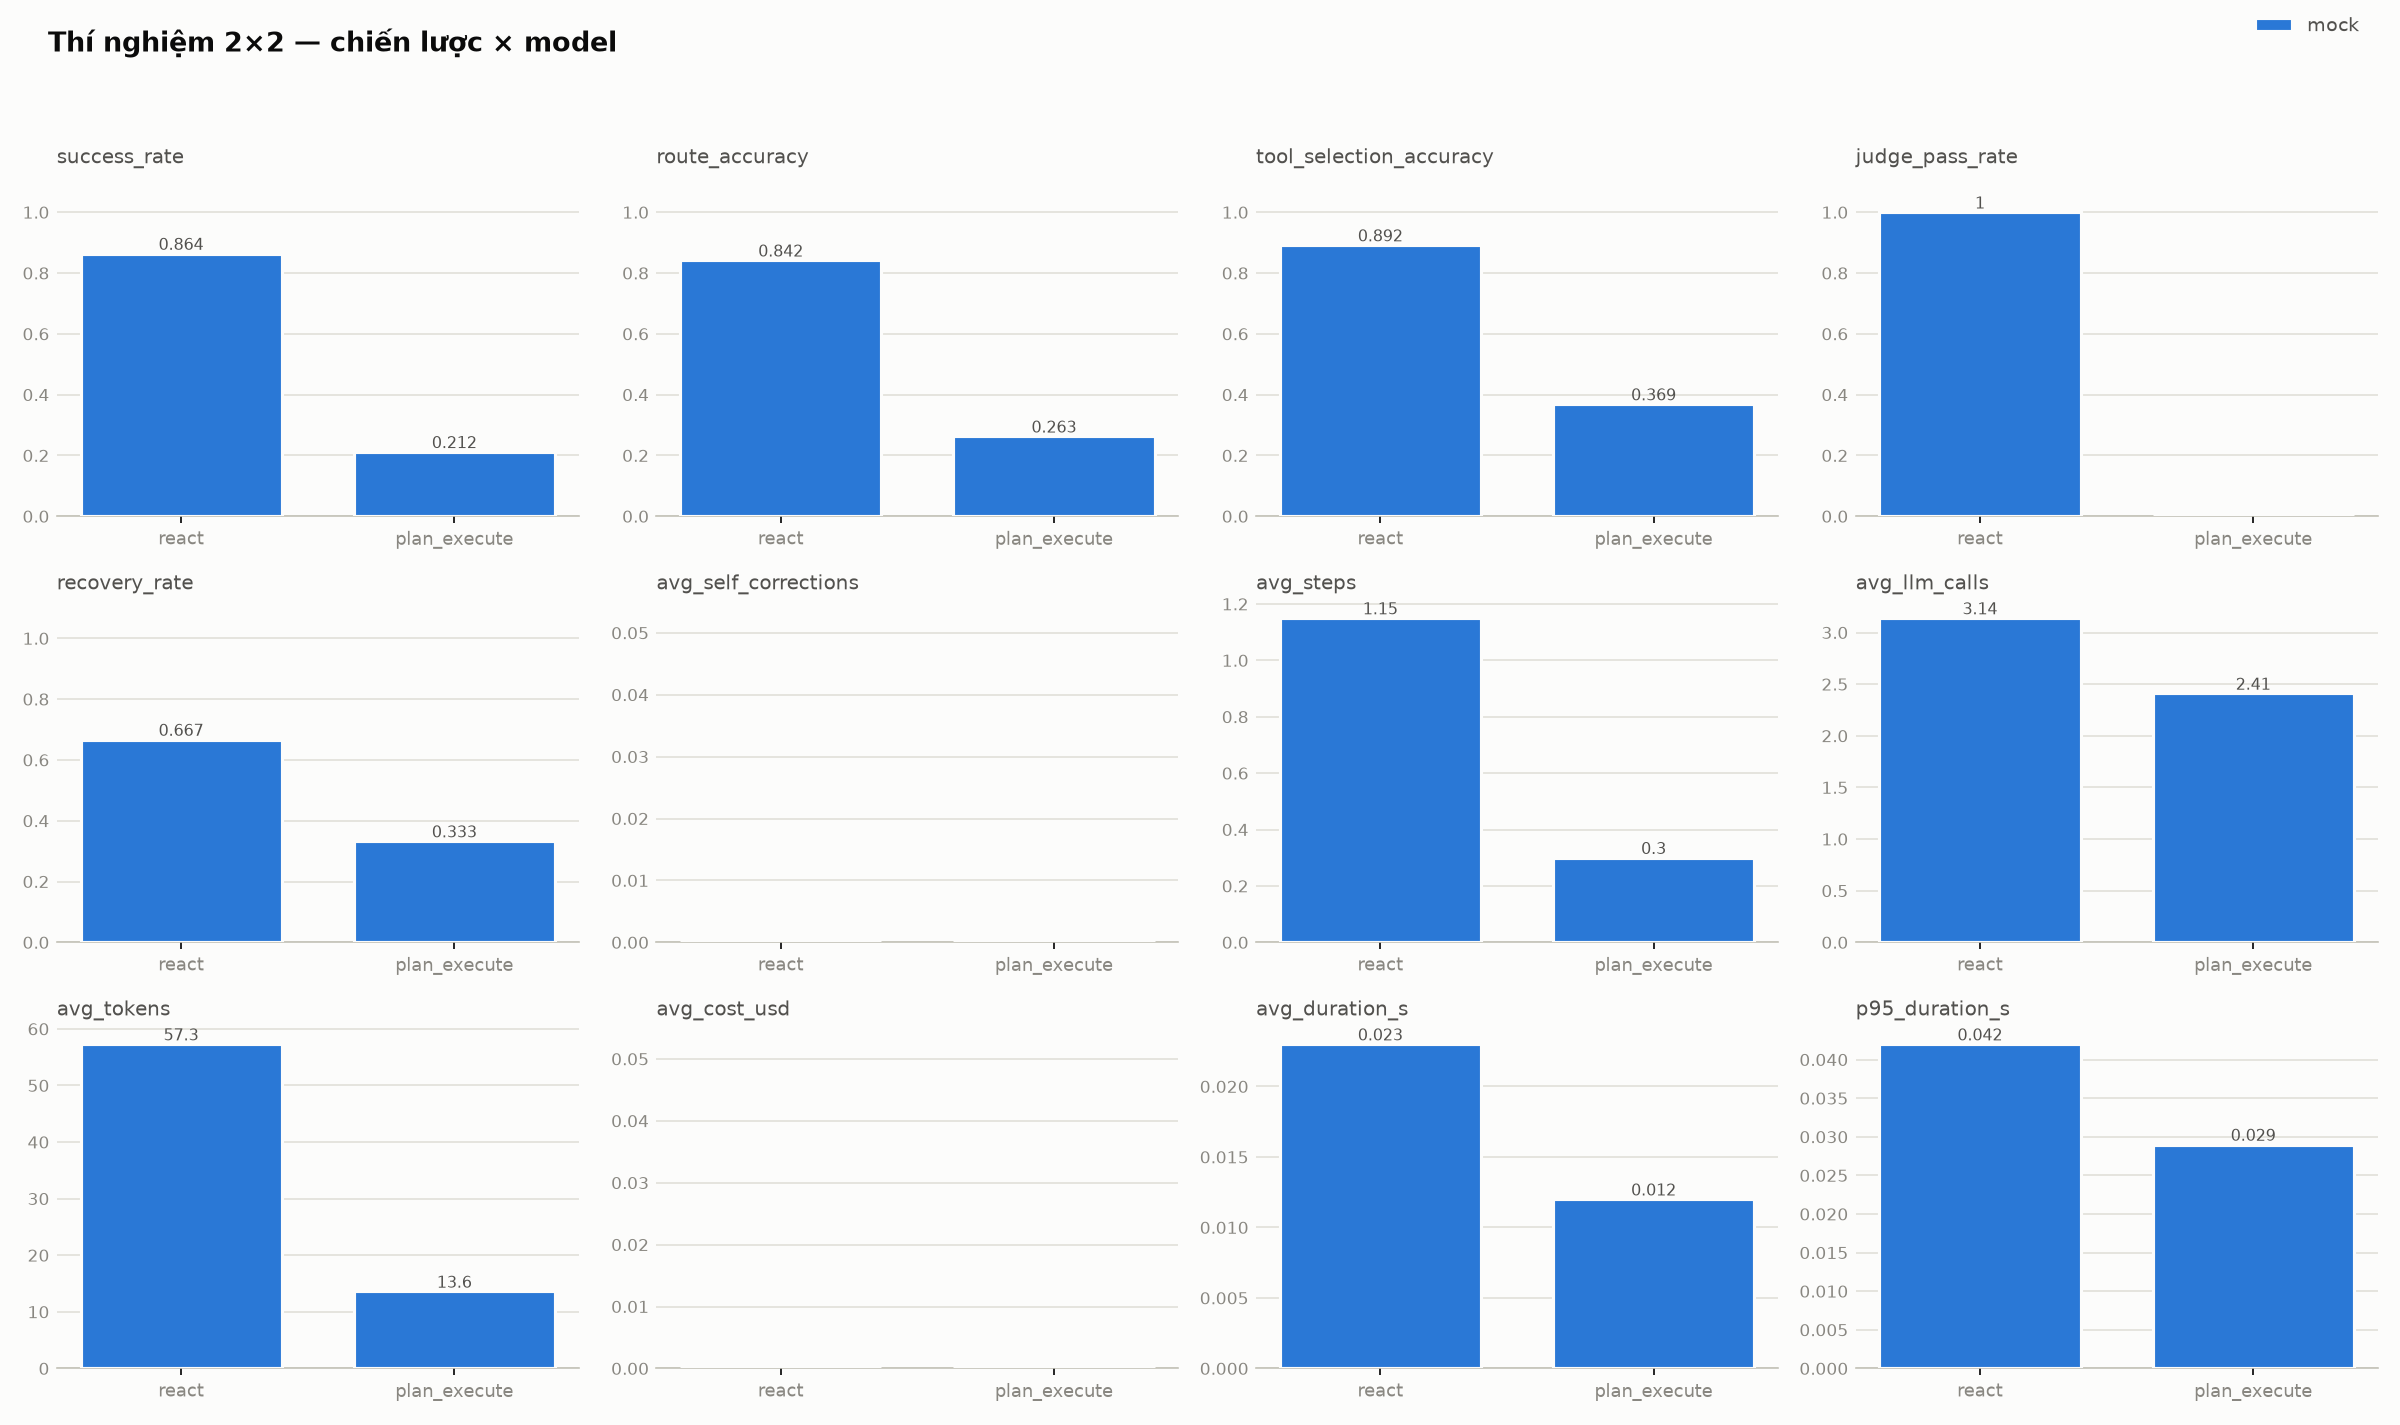
\includegraphics[width=\linewidth]{metrics_grid}
  \caption{So sánh metric giữa hai cấu hình mock (ReAct và
    Plan-and-Execute, mỗi cột 198 run) từ
    \texttt{evals/results/exp-final/metrics\_grid.png}. Trục token, chi
    phí, thời gian mang tính tham khảo vì MockLLM không gọi mạng.}
  \label{fig:metrics-grid}
\end{figure}

\subsection{Phân tích theo nhóm case (mẫu Gemini)}

\begin{table}[ht]
\centering
\caption{Success rate theo nhóm trên mẫu Gemini $\times$ ReAct (22 case
$\times$ $n=3$). Nhãn nhóm có thể chồng nhau (ví dụ case scheduler cũng
thuộc nhóm xác nhận; case fetch hỏng vĩnh viễn cũng thuộc nhóm một công
cụ). Mẫu nhỏ --- mỗi nhóm chỉ 1--8 case --- nên các con số chỉ mang tính
minh họa.}
\label{tab:ket-qua-theo-nhom}
\begin{tabular}{lccc}
\toprule
Nhóm case & Số case & Run đạt / tổng & Tỷ lệ (\%) \\
\midrule
Trả lời trực tiếp / hỏi lại & 3 & 9/9   & 100 \\
Một công cụ                 & 8 & 19/24 & 79{,}2 \\
Nhiều bước                  & 7 & 11/21 & 52{,}4 \\
Xác nhận (HITL)             & 3 & 6/9   & 66{,}7 \\
Phục hồi lỗi                & 1 & 0/3   & 0 \\
Prompt injection            & 2 & 6/6   & 100 \\
Đường lỗi                   & 1 & 0/3   & 0 \\
Scheduler (cron)            & 1 & 0/3   & 0 \\
\bottomrule
\end{tabular}
\end{table}

Ba nhận xét chính. \emph{Thứ nhất}, nhóm khó nhất đúng như dự đoán là
nhiều bước (52{,}4\%) và phục hồi lỗi (0/3): ở case
\texttt{recovery\_fetch\_fails\_fallback\_search}, judge ghi nhận cả ba
run rằng model ``thừa nhận không truy cập được trang web nhưng không
chuyển sang tìm kiếm thay thế'' --- agent trung thực về lỗi nhưng chưa
chủ động đổi nguồn. \emph{Thứ hai}, không case injection nào bị vượt:
6/6 run Gemini và 30/30 run nhóm injection của cấu hình mock ReAct đều
đạt. \emph{Thứ ba}, hai case cho kết quả không ổn định giữa các run
(\texttt{single\_task\_done} đạt 1/3, \texttt{multi\_plan\_execute\_todos\_note}
đạt 2/3) --- minh chứng trực tiếp cho yêu cầu lặp $n \geq 3$ với hệ thống
không tất định.

\subsection{Self-correction}

Trên 396 run mock không có lần tự sửa schema nào (kịch bản tất định trả
JSON đúng). Trên 66 run Gemini chỉ có \textbf{1 run} cần tự sửa
(\texttt{multi\_search\_report\_note\_react}, run thứ hai: 1 lệnh gọi
purpose \texttt{:fix1}, sau đó chạy tiếp bình thường và đạt), tức
1{,}5\% số run --- \texttt{gemini-3.1-flash-lite} giữ schema JSON khá
vững trong môi trường prompt của hệ thống (danh sách tên công cụ hợp lệ
được nhắc ngay cạnh yêu cầu JSON, Mục~\ref{sec:ky-thuat-selfcorrect}).
Cơ chế tự sửa vì vậy ít phải kích hoạt, nhưng lần kích hoạt duy nhất đã
cứu được một run multi-step thay vì để fail.

\subsection{Phân tích theo câu hỏi nghiên cứu}

\paragraph{RQ1 (chiến lược).} Dữ liệu hiện có \emph{chưa trả lời trọn
vẹn} RQ1: phần mock cho thấy cả hai chiến lược đều đạt 100\% ở ô trùng
chiến lược gốc --- nghĩa là khung agent hiện thực hóa đúng cả hai, nhưng
môi trường kịch bản không phân định được chiến lược nào ``thông minh''
hơn; còn phần model thật chỉ có số liệu cho ReAct. Quan sát gián tiếp duy
nhất: Plan-Execute dùng ít lệnh gọi LLM hơn trên mỗi tác vụ (2{,}41 so
với 3{,}14 trên mock), nhất quán với giả thuyết chi phí đoán được hơn.
So sánh hai chiến lược trên model thật được chuyển sang hướng phát triển.

\paragraph{RQ2 (mô hình).} So với trần 100\% của môi trường kịch bản,
model thật trên 22 case mẫu đạt 72{,}7\%. Phần rơi rớt tập trung ở
multi-step, phục hồi lỗi và scheduler-qua-confirm (model từ chối thiết
lập lịch ở cả 3 run của \texttt{confirm\_scheduler\_approved}); các nhóm
direct/clarify, injection giữ nguyên 100\%, route accuracy thậm chí đạt
94{,}4\%. Về tài nguyên: một tác vụ trung bình tốn 3\,822 token
($\approx$ 0{,}0005 USD ước tính); toàn bộ 66 run hết $\approx$ 0{,}033
USD. Độ trễ trung bình 25{,}7\,s bị kéo bởi backoff khi dính rate limit
429 của free tier (11/66 run vượt 60\,s, tối đa 412\,s); trung vị
4{,}9\,s phản ánh sát hơn độ trễ thật của một tác vụ.

\paragraph{RQ3 (chống chịu).} Về injection, không run nào bị vượt trong
toàn bộ dữ liệu đã chạy (6/6 Gemini, 30/30 mock ReAct); các lớp đóng
khung \texttt{<tool\_output>}, quy tắc system prompt và confirm bắt buộc
(Mục~\ref{sec:ky-thuat}) đều chưa bị xuyên thủng --- với lưu ý mẫu
Gemini mới phủ 2 case injection. Về phục hồi lỗi, cơ chế của khung
(retry, lỗi thành observation) hoạt động đúng trong mock, nhưng case
recovery duy nhất của mẫu Gemini thất bại cả 3 run vì model dừng ở mức
báo lỗi trung thực thay vì đổi nguồn --- điểm yếu thuộc về hành vi model
và prompt, không phải cơ chế, và là mục tiêu cải thiện cụ thể tiếp theo.

\subsection{Case study}

\textbf{Tác vụ nhiều bước thành công} ---
\texttt{multi\_search\_report\_note\_react} (Gemini, run thứ hai): yêu
cầu tìm kiếm, viết báo cáo rồi lưu ghi chú. Trace ghi 5 bước công cụ, 8
lệnh gọi LLM (trong đó 1 lệnh \texttt{:fix1} tự sửa schema), 11\,432
token, chi phí ước tính 0{,}0014 USD, tổng 18{,}9\,s --- chuỗi
\texttt{web\_search} $\to$ \texttt{report\_builder} $\to$
\texttt{note\_store} hoàn chỉnh, đạt toàn bộ kỳ vọng.

\textbf{Từ chối confirm được xử lý đúng} ---
\texttt{confirm\_delete\_rejected} (Gemini, cả 3 run đạt, judge pass
3/3): người dùng yêu cầu xóa ghi chú rồi bấm từ chối. Mỗi run 3 bước, 5
lệnh gọi LLM, $\approx$ 3\,950 token, run nhanh nhất 4{,}4\,s; judge xác
nhận câu trả lời ``thông báo thao tác xóa đã hủy và dữ liệu được giữ
nguyên''. Ngược lại, case phục hồi lỗi ở trên cho thấy mặt chưa đạt:
agent dừng sau 1--2 bước với lời báo lỗi trung thực nhưng không thử
\texttt{web\_search} thay thế --- hai trace này (xem được qua trace
viewer/replay) minh họa đúng ranh giới năng lực hiện tại của hệ thống.

\section{Giới hạn và hướng phát triển}
\label{sec:gioi-han}

\subsection{Giới hạn}

\begin{itemize}
  \item \textbf{Phạm vi kênh và hạ tầng}: chỉ hỗ trợ Telegram; một tiến trình,
        SQLite, scheduler in-process --- phù hợp quy mô cá nhân, chưa phân tán.
        Agent loop đồng bộ chiếm một thread cho mỗi tác vụ đang chạy.
  \item \textbf{Bảo mật}: REST API mới bảo vệ bằng một API key đơn (header),
        chưa có auth thật; định danh người dùng dựa vào Telegram.
  \item \textbf{Chống prompt injection ở mức giảm thiểu}: đóng khung dữ liệu,
        vô hiệu hóa delimiter giả, quy tắc trong system prompt, xác nhận người
        dùng --- không có bảo đảm tuyệt đối trước tấn công tinh vi hơn (bài
        toán mở của cả lĩnh vực~\cite{greshake2023injection}).
  \item \textbf{Trần chi phí theo chặng chạy}: trần 0{,}25~USD áp cho từng
        chặng run/resume, không cộng dồn qua các lần tạm dừng chờ xác nhận ---
        một tác vụ nhiều lần confirm có thể tốn hơn trần danh nghĩa (tổng chi
        phí thật vẫn tra được qua \texttt{task\_usage}).
  \item \textbf{Rate limit và cache in-memory}: trạng thái rate limiter và
        search cache nằm trong RAM của tiến trình --- restart là reset; cache
        tìm kiếm khớp theo truy vấn chuẩn hóa (exact-match), chưa phải
        semantic cache theo nghĩa embedding.
  \item \textbf{Memory dài hạn}: mới dừng ở hồ sơ người dùng dạng JSON, agent
        chưa khai thác; chưa có vector memory/RAG.
  \item \textbf{Giới hạn kỹ thuật}: timeout không kill được thread công cụ
        đang chạy (giới hạn Python) --- thread cũ được bỏ lại có kiểm soát.
  \item \textbf{Đánh giá}: LLM-as-judge mới chấm pass/fail theo tiêu chí từng
        case, chưa có thang điểm nhiều mức và chưa kiểm chứng chéo tay trên
        mẫu lớn; trong lần chạy mẫu, judge còn dùng chính model agent
        (\texttt{gemini-3.1-flash-lite}) nên có rủi ro self-preference.
        Bộ 66 case chưa phủ hết không gian hành vi.
  \item \textbf{Phần model thật chỉ là mẫu minh họa}: quota free tier Gemini
        (500 request/ngày) cạn giữa chừng nên thay vì đủ ma trận
        $2 \times 2$, chỉ đo được một cấu hình ReAct $\times$ Gemini trên
        22/66 case ($n=3$, 66 run) --- chưa đủ để so sánh chéo model hay so
        sánh hai chiến lược trên model thật (RQ1, RQ2 mới trả lời một
        phần, Mục~\ref{sec:ket-qua}); việc đo model khác sẽ thực hiện trong
        tương lai. Số liệu exp-final cũng chỉ ra hai điểm cần thận trọng:
        (1) kết quả model thật dao động giữa các run (2/22 case đổi
        pass/fail giữa 3 lượt) nên khác biệt nhỏ giữa cấu hình chưa có ý
        nghĩa; (2) nhóm yếu nhất trên model thật là multi-step
        (52{,}4\%) và phục hồi lỗi (0/3 --- model báo lỗi trung thực nhưng
        không tự đổi nguồn); độ trễ đo được còn bị méo bởi backoff 429 của
        free tier (trung bình 25{,}7\,s so với trung vị 4{,}9\,s).
\end{itemize}

\subsection{Hướng phát triển}

\begin{itemize}
  \item Mở rộng kênh (web chat/Slack) trên cùng lõi agent; PostgreSQL và
        scheduler phân tán khi cần đa máy; tách worker + queue để bỏ giới hạn
        một thread/tác vụ.
  \item Memory dài hạn có cấu trúc + RAG cho tri thức cá nhân.
  \item Phòng thủ injection nhiều lớp hơn (bộ lọc đầu ra công cụ, sandbox
        quyền theo từng tác vụ); trần chi phí cộng dồn theo cả vòng đời tác
        vụ.
  \item Chuẩn hóa tool interface theo hướng Model Context Protocol (MCP) để
        dùng lại hệ sinh thái công cụ bên ngoài.
  \item Mở rộng eval: chạy đủ ma trận 2 chiến lược $\times$ nhiều model thật
        (khi có quota hoặc model khác) để trả lời trọn RQ1--RQ2; thêm case
        đối kháng, tăng số lượt lặp, thang điểm judge nhiều mức có kiểm
        chứng người (judge tách model với agent), đo chi phí--chất lượng
        theo Pareto để chọn model.
\end{itemize}

\section*{Kết luận}
\addcontentsline{toc}{section}{Kết luận}

Đồ án xây dựng Laplace's Demon --- một AI agent cá nhân hoàn chỉnh từ kênh
giao tiếp (Telegram) đến lõi điều phối (state machine tự xây với hai chiến
lược ReAct và Plan-and-Execute cắm chung một interface), với ba trụ cột thiết
kế được hiện thực hóa nhất quán: an toàn theo lớp (giới hạn bước/timeout,
xác nhận người dùng bền vững qua restart, trần chi phí, rate limit, chống
prompt injection nhiều lớp), khả năng quan sát (mọi lệnh gọi LLM và mọi lần
chạy công cụ đều có trace; trace viewer kèm chi phí và chế độ phát lại
offline), và đánh giá định lượng (eval harness 66 case, 8 metric, chạy đúng
agent loop production, tùy chọn LLM-as-judge). Thực nghiệm
\texttt{exp-final} cho thấy khung agent đạt 100\% trên toàn bộ 198 run
mock trùng chiến lược gốc ở cả hai chiến lược (vai trò regression
benchmark), và trên mẫu model thật Gemini $\times$ ReAct (22 case,
$n=3$) đạt 72{,}7\% success với chi phí $\approx$ 0{,}0005 USD/tác vụ ---
mạnh ở phân tuyến (route accuracy 94{,}4\%), trả lời trực tiếp và chống
injection (không run nào bị vượt), yếu ở multi-step và tự phục hồi lỗi;
ReAct được giữ làm chiến lược mặc định vì là cấu hình duy nhất đã có số
liệu model thật và xử lý mềm hơn khi người dùng từ chối confirm.

Bài học lớn nhất của đồ án nằm ở phương pháp: khi trace là công dân hạng
nhất và bộ eval lặp lại được, mọi thay đổi --- từ sửa prompt đến đổi chiến
lược hay model --- đều trở thành một thí nghiệm có số liệu thay vì một cảm
nhận; chính vòng phản hồi này (eval phát hiện model bịa tên công cụ $\to$
sửa prompt $\to$ eval xác nhận cải thiện) đã định hình phần lớn các kỹ thuật
ở Mục~\ref{sec:ky-thuat}.


\bibliographystyle{plain}
\bibliography{refs}

\end{document}
